\subsection{階層型NNによる学習}
\subsubsection{最適なパラメータを探すためのアプローチ}
指定された条件下において学習が効率良く行われるパラメータの組み合わせを探
すため、他の値をそのままにALPHAの値を0.1刻みで変更して最も収束にかかった回数の少ないものを求める。以降ALPHAをその値で固定して,ETAを0.1刻みで変更していき,最も収束にかかった回数の少ないものを求める。その後,HIDDENの上限を50にして1刻みで変更していき,最も収束にかかった回数の少ないものを求める。以上のようにすることで最も良いパラメータを調整した。HIDDENの総当たりの際に使用したスクリプトを以下に示す(ソースコード\ref{hidden}).

\lstinputlisting[caption=lv2-HIDDEN.pl,label=hidden]{../nn/bp_mo/lv2-HIDDEN.pl}

\subsubsection{実行結果}
上記のアプローチのようにパラメータを求めた際,

ETA=1.9,ALPHA=0.9,HIDDEN=15

となった。

この値を用いてシード値10パターン結果が表\ref{table:level2},その10パターンの平均を取ったグラフが以下の図\ref{fig:level2}である。

\begin{table}[htb]
 \begin{center}
  \caption{階層型NNによるExOR問題の学習に要した回数}
  \label{table:level2}
  \begin{tabular}[htb]{r|l} \hline
   シード値 & 収束した回数 \\ \hline \hline
   1000 & 48 \\ \hline
   2000 & 66 \\ \hline
   3000 & 88 \\ \hline
   4000 & 66 \\ \hline
   5000 & 57 \\ \hline
   6000 & 62 \\ \hline
   7000 & 49 \\ \hline
   8000 & 34 \\ \hline
   9000 & 50 \\ \hline
   10000 & 44 \\ \hline \hline
   10試行の平均値 & 56.4 \\ \hline
  \end{tabular}
 \end{center}
\end{table}

\begin{figure}[h]
 \begin{center}
  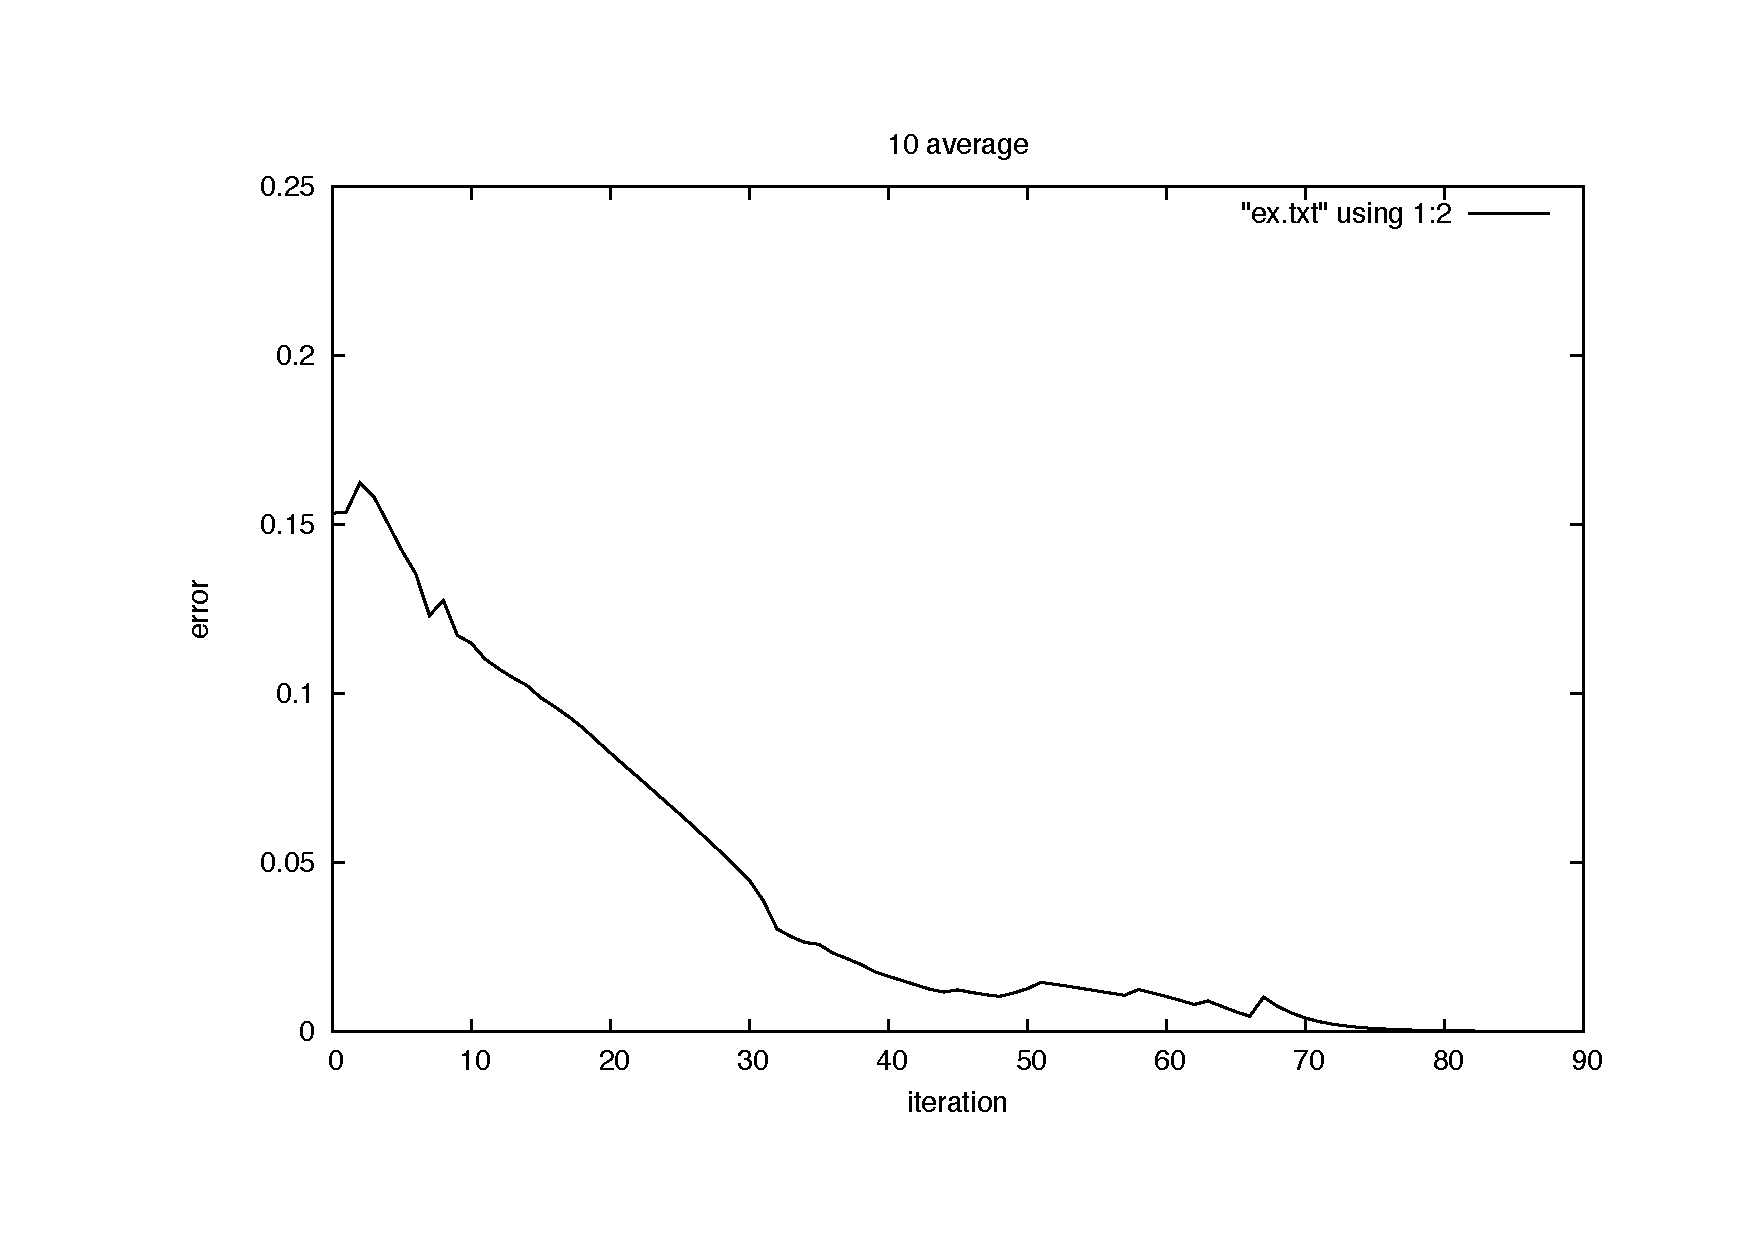
\includegraphics[width=10.0cm,angle=-90]{figs/level2/ave1.pdf}
  \caption{重みを更新する様子(平均値)}
  \label{fig:level2}
 \end{center}
\end{figure}


\subsubsection{考察}
今回の実行では,ETAの値が1.9,ALPHAの値が0.9,HIDDENの値が15となる場合に最も学習が効率よく収束することがわかった。今回,ETAの値が大きくなるごとに効率が良くなった。これは前回の実験からも分かるように学習係数が大きくなるごとに学習速度は上がるためであると考える。さらにALPHAの値も大きくなるごとに効率が良くなった。調べて見たところ,学習速度を上げるために慣性項を付与する方法があり,それをモーメント法と呼ぶようである。このモーメント法は,慣性項の値が1に近い方が良いとされる。HIDDENの値は今回1から50までを全て試したが,結果がバラバラであり,規則性はないのではないかと考える。よって,これらの値を全て効率の良い組み合わせにするためには相当根気のいる作業が必要なのではないかと思われる。

